\documentclass[10pt, compress]{beamer}

\usetheme[usetitleprogressbar]{m}

\usepackage{booktabs}
\usepackage{amsmath}
\usepackage{nicefrac}
\usepackage{color}
\usepackage{wrapfig}

\title{HAUM}
\subtitle{\alert{H}ackerspace \alert{au M}ans}
\date{Oct. 2015}
\author{}
\institute{HAUM}

\begin{document}

\maketitle

\begin{frame}[fragile]
	\frametitle{Le HAUM en 5 lignes}

	\begin{itemize}
		\item \alert{30+} membres
		\item \alert{3 ans} d'existence
		\item \alert{50} dépôts de code sur Github
		\item \alert{4} formations sur Arduino, Git, etc...
		\item \alert{4} projets autour de la lumière
	\end{itemize}
\end{frame}

\section{Les Projets}

\begin{frame}[fragile]
	\frametitle{Les projets en bref : AxiHAUM \& PCBlastifieuse}

	\begin{itemize}
		\item \alert{Axihaum} : réparation \& modification d'une fraiseuse à PCB, utilisation de LinuxCNC, contributions à HeeksCAD/CNC
		\item \alert{PCBlastifieuse} : modification d'une plastifieuse pour des PCB de bonne qualité
		\item Création d'outils
	\end{itemize}

	\begin{center}
		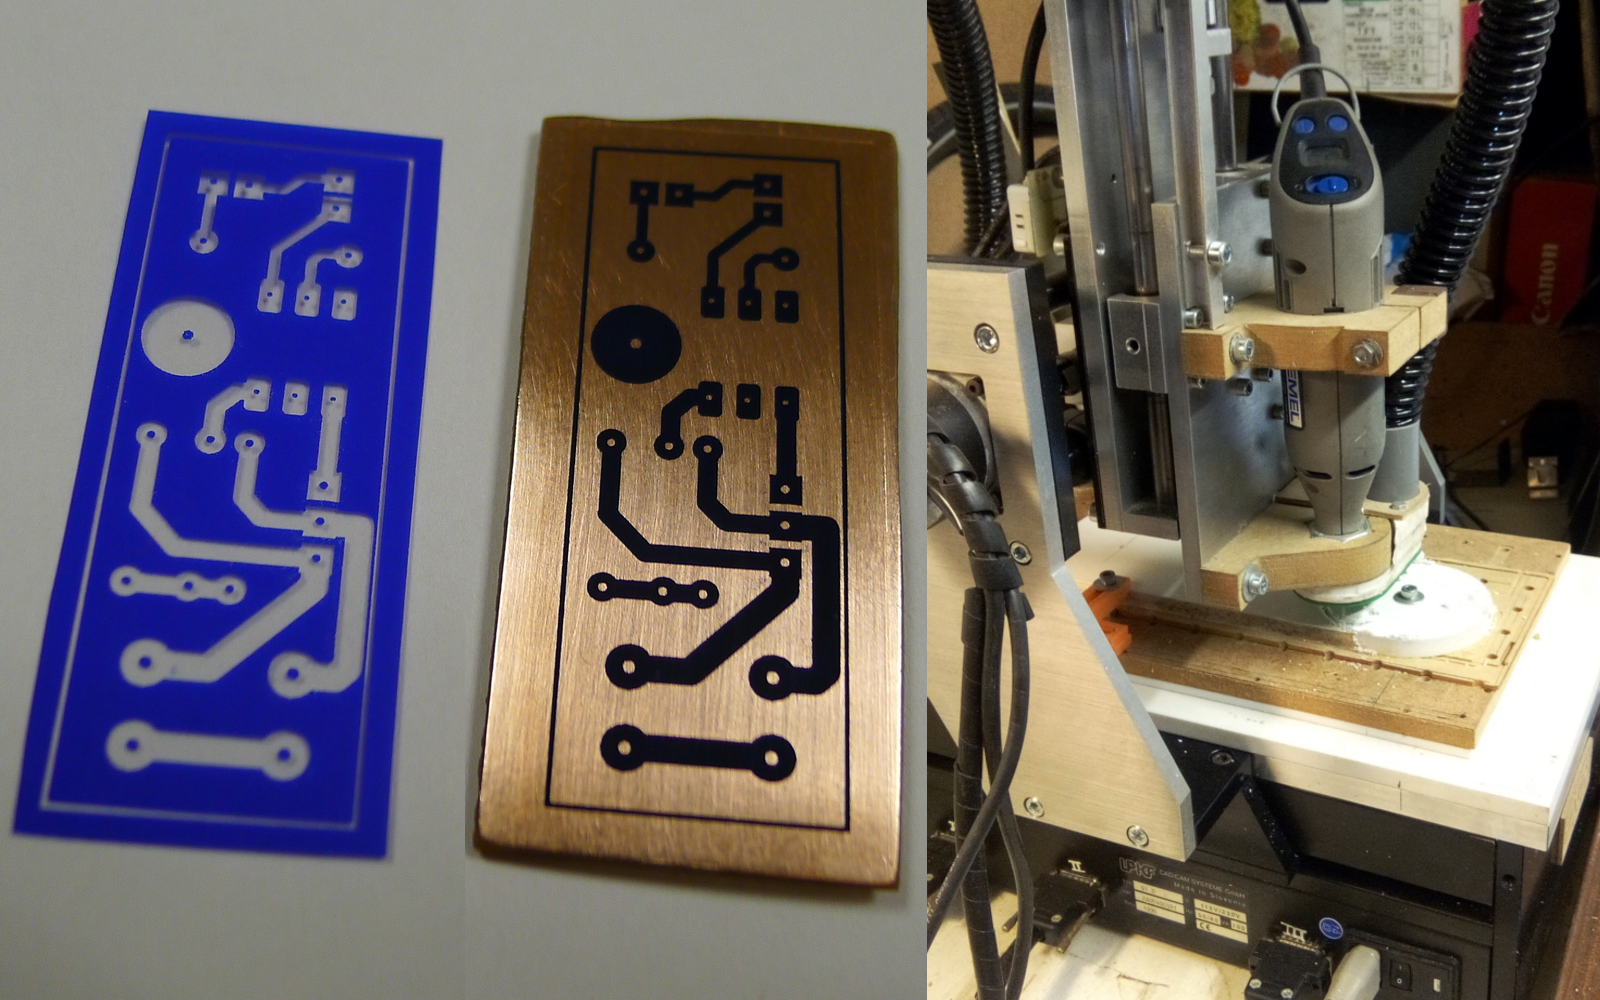
\includegraphics[width=0.6\textwidth]{axihaum_pcb.png}
	\end{center}
\end{frame}

\begin{frame}[fragile]
	\frametitle{Les projets en bref : OpenData}

	\begin{itemize}
		\item \alert{Dataélections} : Récupération, traitement et affichage de données électorales
		\item \alert{timeoapi} : Création d'API pour des services utiles (SETRAM, etc...)
		\item Démarche citoyenne
	\end{itemize}

	\begin{center}
		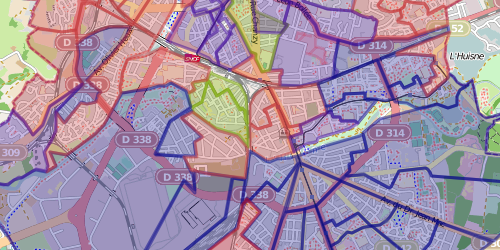
\includegraphics[width=0.9\textwidth]{europeenes.png}
	\end{center}
\end{frame}

\begin{frame}[fragile]
	\frametitle{Les projets en bref : Musique}

	\begin{itemize}
		\item \alert{dHAUMidi} : instrument à taille humaine multi-utilisateurs
		\item \alert{PianoStairs} : animation d'escalier à moindres frais
		\item Projets ludiques \& innovants
	\end{itemize}

	\begin{center}
		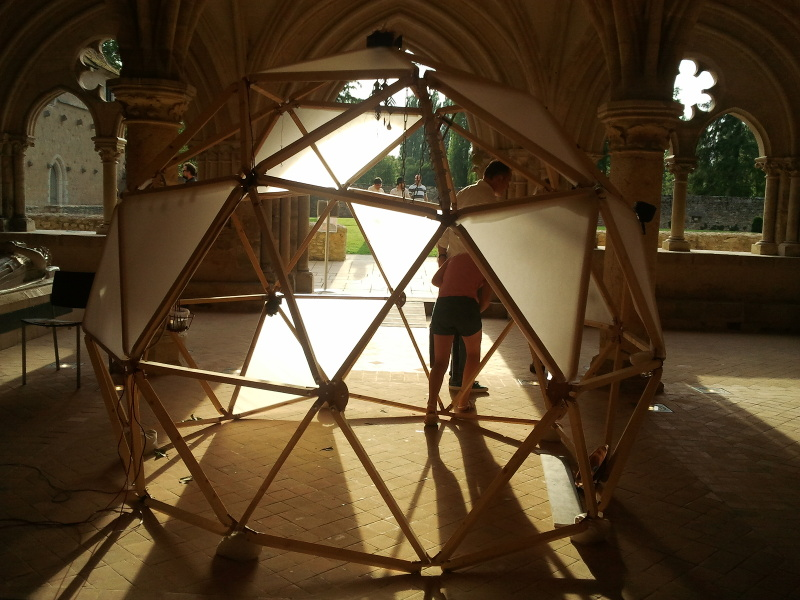
\includegraphics[width=0.6\textwidth]{dhaum.png}
	\end{center}
\end{frame}

\begin{frame}[fragile]
	\frametitle{Les projets en bref : Polychrhaum \& Cie.}

	\begin{itemize}
		\item \alert{1D Pong} : jeu minimaliste en 1 dimension sur une bande de LEDs
		\item \alert{HAUMTinsel} : jeu multijoueurs sur guirlande avec interface web
		\item Et tant d'autres...
	\end{itemize}

	\begin{center}
		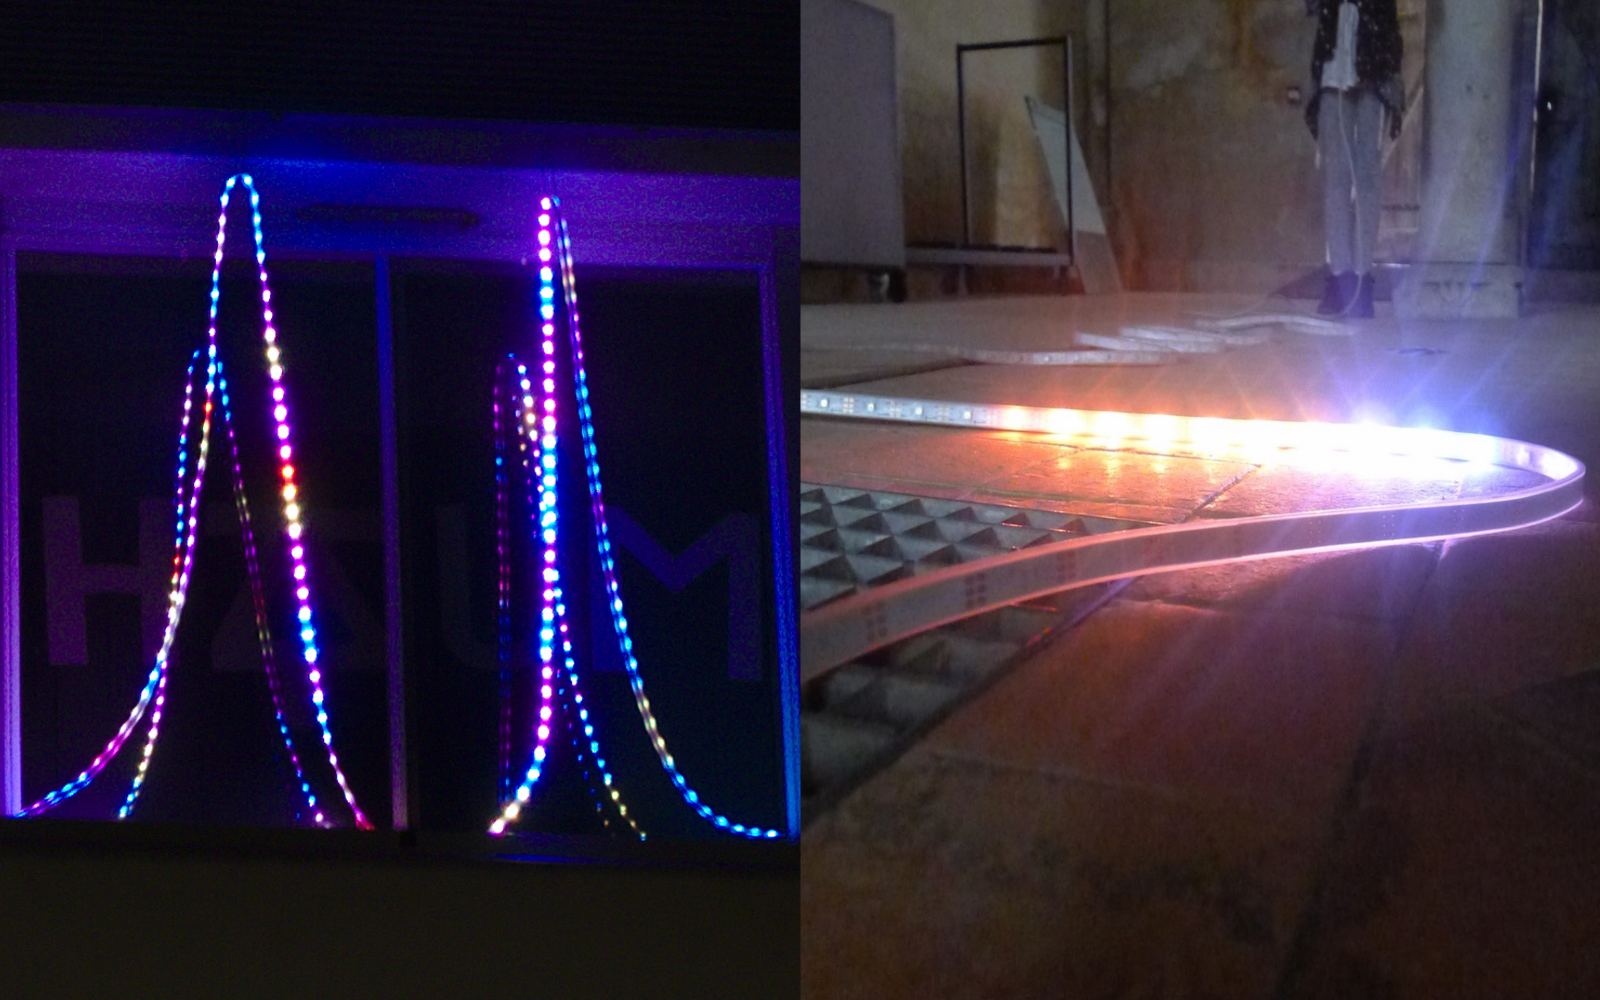
\includegraphics[width=0.6\textwidth]{lights.png}
	\end{center}
\end{frame}

\section{Projet de Noël}

\begin{frame}
	\frametitle{Projet de Noël}

	\alert{\textsc{Idée} :} exploiter les guirlandes en place pour animer la ville

	\pause

	Plusieurs jeux possibles :

	\begin{itemize}[<+->]
		\item Une ré-écriture de \alert{HAUMTinsel} à plus grande échelle
		\item Une ré-écriture du \alert{Pong} à plus grande échelle
		\item Un jeu multi-équipes type \alert{«zone»} sur le centre ville
		\item Des \alert{jeux ponctuels} en centre ville
	\end{itemize}
\end{frame}

\begin{frame}[fragile]{Projet de Noël : Objectifs}

	\textbf{Plusieurs avantages...}

	\pause

	\begin{itemize}[<+->]
		\item Des \alert{retombées économiques} possibles (avec les commerçants du centre)
		\item Une plus grande \alert{fréquentation} du centre ville par un \alert{autre public}
		\item Un vecteur de \alert{communication} pour Le Mans et les réalisateurs du projet
		\item Une \alert{expérience} d'un nouveau type de \alert{décorations interactives}
	\end{itemize}
\end{frame}

\plain{Merci !\\
\vspace{0.25\textwidth}
Des questions ?\\
\vspace{0.15\textwidth}
\scriptsize{\texttt{mathieu@haum.org}}
}

\end{document}
